\documentclass[12pt, a4paper]{report}
\usepackage{style}


\title{Numerical Analysis \\ \textit{Theory}}
\author{Christian Rossi}
\date{Academic Year 2023-2024}

\begin{document}

\maketitle

\newpage

\begin{abstract}
The topics of the course are:
\begin{itemize}
    \item Floating-point arithmetic: different sources of the computational error; absolute vs relative errors; the floating point representation 
        of real numbers; the round-off unit; the machine epsilon; floating-point operations; over- and under-flow; numerical cancellation.
    \item Numerical approximation of nonlinear equations: the bisection and the Newton methods; the fixed-point iteration; convergence analysis 
        (global and local results); order of convergence; stopping criteria and corresponding reliability; generalization to the system of 
        nonlinear equations (hints).
    \item Numerical approximation of systems of linear equations: direct methods (Gaussian elimination method; LU and Cholesky factorizations; 
        pivoting; sparse systems: Thomas algorithm for tridiagonal systems); iterative methods (the stationary and the dynamic Richardson scheme; 
        Jacobi, Gauss-Seidel, gradient, conjugate gradient methods (hints); choice of the preconditioner; stopping criteria and corresponding 
        reliability); accuracy and stability of the approximation; the condition number of a matrix; over- and under-determined systems: the 
        singular value decomposition (hints).
    \item Numerical approximation of functions and data: Polynomial interpolation (Lagrange form); piecewise interpolation; cubic interpolating 
        splines; least-squares approximation of clouds of data.
    \item Numerical approximation of derivatives: finite difference schemes of the first and second order; the undetermined coefficient method.
    \item Numerical approximation of definite integrals: simple and composite formulas; midpoint, trapezoidal, Cavalieri-Simpson quadrature rules; 
        Gaussian formulas; degree of exactness and order of accuracy of a quadrature rule. 
    \item Numerical approximation of ODEs: the Cauchy problem; one-step methods (forward and backward Euler and Crank-Nicolson schemes); 
        consistency, stability, and convergence (hints).
\end{itemize}
\end{abstract}

\newpage

\tableofcontents

\newpage

\chapter{Introduction}
    \section{Numerical analysis and errors}
    Numerical analysis is the branch of mathematics concerned with employing electronic calculators to discover solutions for specific mathematical problems. 
    It represents the fusion of mathematical principles and computer science.
    On the other hand, scientific computing also involves the formalization of models, requiring a foundation in engineering knowledge.
    \begin{figure}[H]
        \centering
        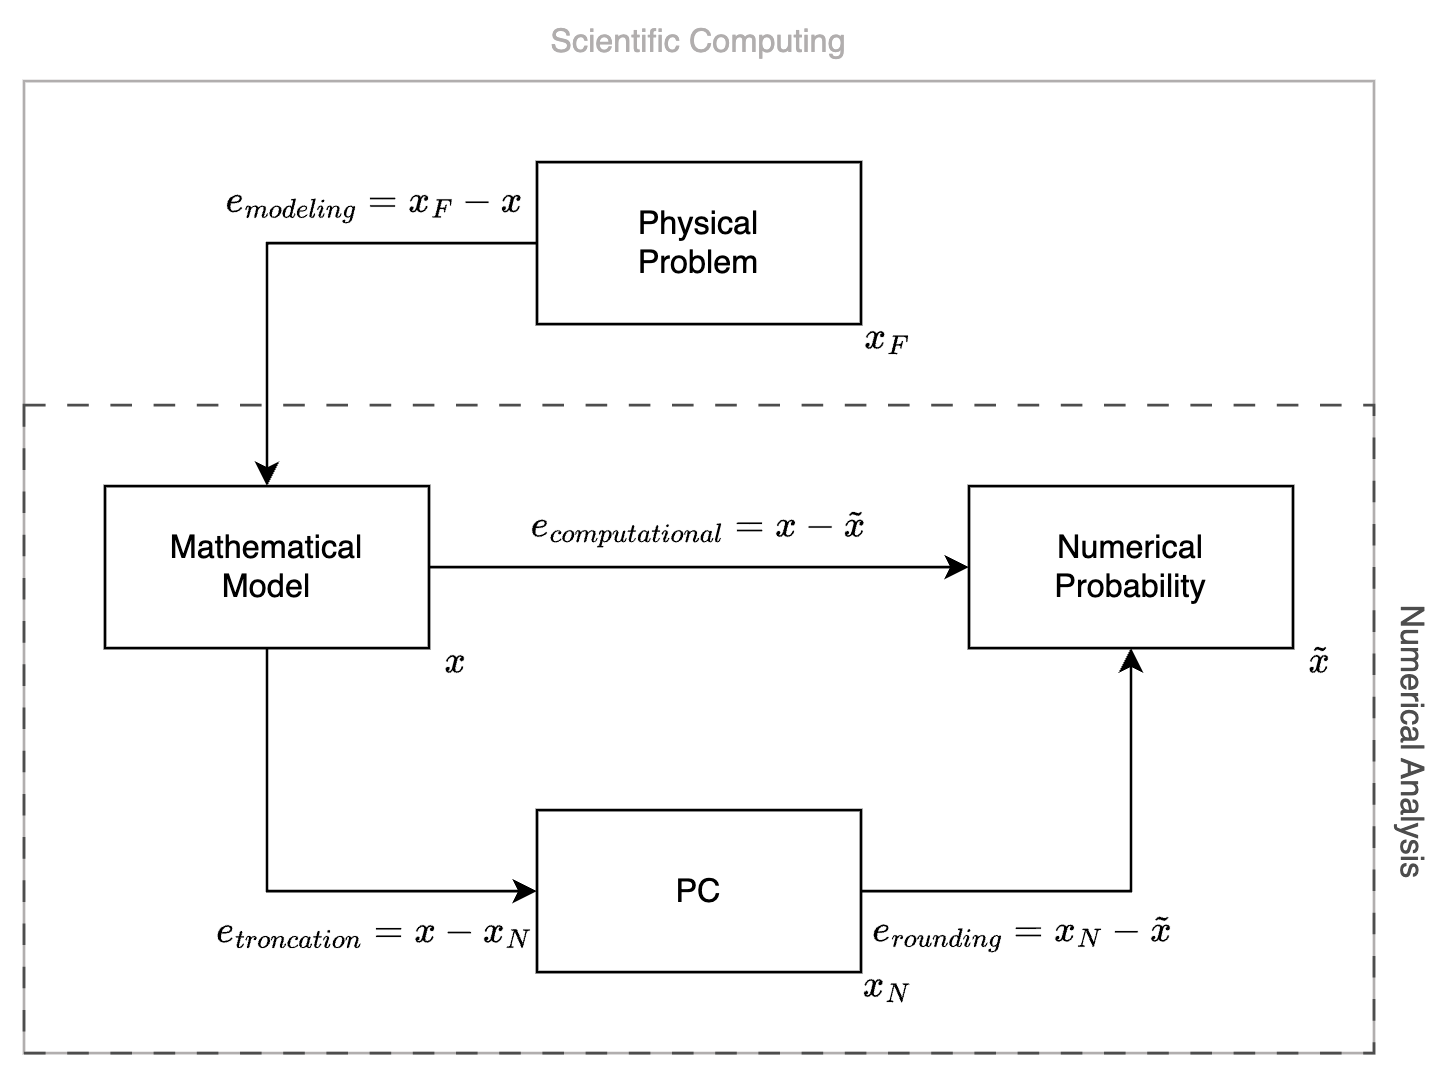
\includegraphics[width=0.75\linewidth]{images/difference.png}
        \caption{Difference between numerical analysis and scientific computing}
    \end{figure}
    As evident in the diagram, each computational step encounters errors. These errors can be categorized into two types:
    \begin{itemize}
        \item Absolute: $\left\lvert x - \tilde{x} \right\rvert$
        \item Relative: $\dfrac{\left\lvert x - \tilde{x} \right\rvert}{\left\lvert x \right\rvert}$, where $x \neq 0$
    \end{itemize}
    The relative error is considered more precise as it relates the error to the measured quantity.
    \begin{example}
        Let's take $x=100$ and $\tilde{x}=100.1$. 
        In this case, the errors are as follows:
        \[e_{abs}=\left\lvert x - \tilde{x} \right\rvert=\left\lvert 100 - 100.1 \right\rvert=0.1\]
        \[e_{rel}=\dfrac{\left\lvert x - \tilde{x} \right\rvert}{\left\lvert x \right\rvert}=\dfrac{\left\lvert 100 - 100.1 \right\rvert}{\left\lvert 100 \right\rvert}=0.001\]
        Now, consider $x=0.2$ and $\tilde{x}=0.1$. 
        In this case, the errors are as follows:
        \[e_{abs}=\left\lvert x - \tilde{x} \right\rvert=\left\lvert 0.2 - 0.1 \right\rvert=0.1\]
        \[e_{rel}=\dfrac{\left\lvert x - \tilde{x} \right\rvert}{\left\lvert x \right\rvert}=\dfrac{\left\lvert 0.2 - 0.1 \right\rvert}{\left\lvert 0.2 \right\rvert}=0.5\]
        The results show that in both examples, the absolute error is the same (0.1), which represents a $10\%$ error. 
        However, the relative error differs significantly.
        In the second example, the relative error is $50\%$, while in the first example, it is only $0.1\%$. 
    \end{example}

    \section{Floating point}
    A finite set of machine numbers, denoted as $\mathbb{F}=\{-\tilde{a}_{min},\dots,\tilde{a}_{max}\}$ and referred to as floating-point numbers, is employed by calculators due to their limited capacity to store numbers and perform operations.
    The process of mapping a real number from the set $\mathbb{R}$ to a value in $\mathbb{F}$ is achieved using the function $fl(x)$, which involves both truncation and rounding operations.

    The set $\mathbb{F}=\mathbb{F}(\beta,t,L,U)$ is defined by four parameters: $\beta,t,L$ and $U$. 
    These parameters collectively characterize every real number $fl(x) \in \mathbb{F}$, which can be expressed as:
    \[fl(x)=(-1)^s(0.a_1a_2\dots a_t)\beta^e\]
    Here's what each component represents:
    \begin{itemize}
        \item $\beta \geq 2$ is the base, an integer determining  the numeric system. 
        \item $m=(0.a_1a_2\dots a_t)$ represents the mantissa.
        \item $e \in \mathbb{Z}$ is the exponent, subject to the constraints $L<e<U$, with $L<0$ and $U>0$. 
        \item $s=\{0,1\}$ denotes the sign.
    \end{itemize}
    In defining the numbers in the mantissa set, a crucial condition is that $a_1 \neq 0$ to ensure the uniqueness of the representation. 
    In such cases, the number is referred to as normalized.

    The set of floating-point numbers exhibits several characteristic values and properties:
    \begin{itemize}
        \item Machine epsilon: it represents the gap between 1 and the smallest floating-point number greater than 1, and it is given by the formula:
            \[\varepsilon_M=\beta^{1-t}\]
        \item Round-off error: this error reflects the relative error introduced when replacing a real number $x \in \mathbb{R}-\{0\}$ with its corresponding $fl(x) \in \mathbb{F}$. 
            It is bounded by the condition:
            \[\dfrac{\left\lvert x-fl(x) \right\rvert}{\left\lvert x \right\rvert }\leq \dfrac{1}{2}\varepsilon_M\]
            where $x \neq 0$.
        \item The biggest and the smallest numbers in the set: these can be calculated using the following formulas:
            \[x_{min}=\beta^{L-1}\]
            \[x_{max}=\beta^U(1-\beta^{-t})\]
    \end{itemize}
    \begin{example}
        In MATLAB, the floating-point set is defined with the following parameters:
        \[(\beta=2,t=53,L=-1021,U=1024)\] 
        With the command "eps" we can find the machine epsilon, that in MATLAB case is:
        \[\epsilon_M=2.22 \cdot 10^{-16}\]
        With the command "realmin" and "realmax" we can find the smallest and the largest numbers representable that are equal to:
        \[x_{min}=2.225073858507201 \cdot 10^{-308}\]
        \[x_{max}=1.797693134862316 \cdot 10^{308}\]
    \end{example}
    An important observation is that not all real numbers are representable in the floating-point set, resulting in a lack of continuity in the latter. 
    Increasing the magnitude of numbers in $\mathbb{R}$ also leads to an increase in the gap between consecutive numbers in $\mathbb{F}$. 
    \begin{example}
        Let us consider the floating number set $\mathbb{F}(2,2,-1,2)$. 
        The characteristic values of this set are: 
        \begin{itemize}
            \item $\epsilon_M=\beta^{1-t}=0.5$.
            \item $x_{min}=\beta^{L-1}=0.25$.
            \item $x_{max}=\beta^U(1-\beta^t)=3$.
            \item $\#\mathbb{F}=2 \beta^{t-1}(\beta -1)(U-L+1)+1=16$. 
        \end{itemize}
        The exponent can take values of $-1,0,1$ and $2$, and the mantissa is represented as $(a_1a_2)_{\beta}$ due to $t=2$. 
        A figure illustrates the possible positive values in this set.
        \begin{figure}[H]
            \centering
            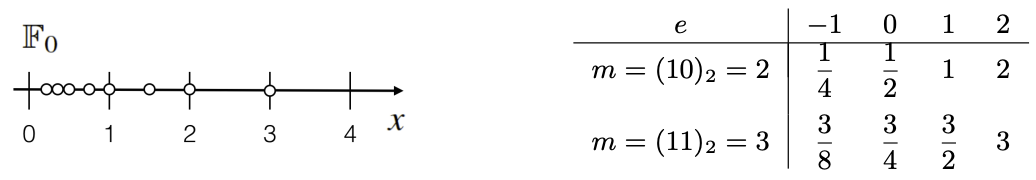
\includegraphics[width=0.9\linewidth]{images/numbers.png}
        \end{figure}
    \end{example}
    One notable consequence of transitioning between the two sets ($\mathbb{R}$ and $\mathbb{F}$) is the loss of two essential properties: associativity and the neutral element for addition.

\newpage 

\chapter{Nonlinear equations}
    \section{Introduction}
    To find a solution for a nonlinear equation $f(x)$, we aim to determine $\alpha \in \mathbb{R}$ that serves as a root of $f$ such that $f(\alpha)=0$.
    \begin{definition}
        A point $\alpha$  is termed a \emph{zero with multiplicity m} if the following conditions are met:
        \begin{itemize}
            \item $f(\alpha)=f^{'}(\alpha)=\dots=f^{\left(m-1\right)}(\alpha)=0$.
            \item $f^{\left(m\right)}(\alpha) \neq 0$.
        \end{itemize}
    \end{definition}
    When $m$ is an odd number, the function exhibits a change in sign as it crosses the zero. 
    In contrast, when $m$ is even, the function maintains the same sign and does not undergo a sign change.

    \section{Iterative methods}
    The set comprising all polynomials of degree $n$ is represented by the symbol $\mathbb{P}_n$ encompassing all polynomials with degrees less than or equal to $n$.
    \begin{theorem}
        There is no solution in radicals to general polynomial equations of degree five or higher with arbitrary coefficients. 
    \end{theorem}
    Therefore, for polynomials with degrees exceeding four, iterative methods are required for solutions. 
    The fundamental concept of these methods can be outlined as follows:
    \begin{enumerate}
        \item Begin with an initial guess, denoted as $x^{(0)}$, which serves as a speculative value for $\alpha$.
        \item Utilize this selected value as an input for a black-box function.
        \item Take the output of the black-box function as the new $x^{(0)}$ and return to step one. 
    \end{enumerate}
    After several iterations, a sequence of values $\{ x^{(n)} \}$ converges such that:
    \[ \lim_{n \rightarrow \infty} = \alpha\]
    Additionally, the error associated with the approximated value for $\alpha$ approaches zero:
    \[ \lim_{n \rightarrow \infty}e^n = 0\]
    This implies that the error can also be expressed as: 
    \[e^n=\alpha-x^{(n)}\]
    All the methods we are going to discuss generate a sequence $x^{(1)},x^{(2)},\dots,x^{(n)}$ of numbers that ideally converges to $\alpha$:
    \[ \lim_{k \rightarrow + \infty} \left\lvert x^{(k)}-\alpha \right\rvert =0\]
    \begin{definition}[order of convergence]
        An iterative method for approximating the zero $\alpha$ of the function $f(x)$ is considered to have a convergence order $q$ if and only if for $k > k_0$:
        \[\left\lvert x^{(k)} - \alpha \right\rvert \leq c {\left\lvert x^{(k+1)} - \alpha \right\rvert}^q  \]
        There are two possible cases:
        \begin{itemize}
            \item If $q=1$, it is termed linear convergence, with the constraint $0<c<1$.
            \item If $q>1$, $c$ can be any positive number greater than zero.
        \end{itemize}
    \end{definition}

    \section{Stopping conditions}
    Iterative methods necessitate a stopping criterion to determine when to halt the iteration process. 
    This criterion can be based on one of four possible conditions:
    \begin{itemize}
        \item Error criterion: terminate if the absolute error satisfies $\left\lvert x^{(k)}-\alpha \right\rvert \leq \epsilon_e$.
        \item Residual criterion: Halt the process if the absolute value of the function's residual meets the condition $\left\lvert f\left(x^{(k)}\right) \right\rvert \leq \epsilon_r$. 
        \item Step length criterion: stop the iteration when the absolute difference between consecutive steps adheres to $\left\lvert x^{(k)}-x^{(k-1)} \right\rvert \leq \epsilon_s$. 
        \item Maximum iterations criterion: terminate the iterations if the number of iterations reaches or exceeds a specified maximum value $k_{max}$. 
    \end{itemize}
    If none of the first three stopping criteria are satisfied, it indicates a lack of convergence in the iterative process.

    \newpage
    \section{Bisection method}
    \begin{theorem}
        Let $f(x)$ be a continuous function on the interval $I=(a,b)$, that is $f \in C^0([a,b])$. 
        If $f(a)f(b)<0$, then there exists at least one zero $\alpha \in I$ of $f(x)$. 
    \end{theorem}
    Suppose there exists a unique zero, denoted as $\alpha$. 
    The bisection method employs a strategy involving the given interval and selects sub-intervals within which the function $f$ exhibits a change in sign.
    By following this procedure, it is assured that each interval chosen in this manner will encompass $\alpha$. 
    
    The sequence $\{x^{(k)}\}$ consisting of the midpoints of these sub-intervals will inevitably converge to $\alpha$. 
    This convergence occurs because the lengths of these sub-intervals decrease to zero as $k$ approaches infinity.
    We can establish the following relationship:
    \[\left\lvert x^{(k)} - \alpha \right\rvert \leq \dfrac{1}{2} \left\lvert b^{(k)}-a^{(k)} \right\rvert \]
    Given the similarity between the left-hand side of this equation and the condition for the error, we can determine the stopping criterion as follows:
    \[\left\lvert b^{(k)}-a^{(k)} \right\rvert \leq 2 \epsilon_e\]
    Now, with the tolerance $\epsilon$ at our disposal, we can calculate the minimum number of iterations required:
    \[k_{min}= \left\lceil {\log_2{\left( \dfrac{\left\lvert b-a \right\rvert}{\epsilon} \right)}-1}\right\rceil\]

    \subsection{Algorithm}
    The algorithm takes as input a continuous function $f$ belonging to $C(\mathbb{R})$ and an interval $[a,b]$ with the property that $f(a)f(b) \leq 0$. 
    The output of the algorithm is an approximate value for the zero of the function.
    \begin{algorithm}[H]
        \caption{Algorithm for the bisection method}
            \begin{algorithmic}[1]
                \For {$k=0,1,\dots,n$}
                    \State $x^{(k)}=\dfrac{a+b}{2}$
                    \If {$\left\lvert b^{(k)}-a^{(k)} \right\rvert \leq 2 \epsilon_e$}
                        \State \Return $x^{(k)}$
                    \ElsIf {$f(x^{(k)})f(a) < 0$}
                        \State $b \leftarrow x^{(k)}$
                    \Else 
                        \State $a \leftarrow x^{(k)}$
                    \EndIf
                \EndFor
            \end{algorithmic}
    \end{algorithm}
    
    \subsection{Summary}
    The advantages of this method are as follows:
    \begin{itemize}
        \item I can control the maximum allowable error.
        \item Convergence is assured.
        \item It relies solely on the evaluation of $f$
    \end{itemize}
    However, there are some drawbacks:
    \begin{itemize}
        \item It is effective only when $f$ changes sign within the interval.
        \item Convergence tends to be slow.
    \end{itemize}
   
    \section{Newton method}
    The bisection method relies solely on the sign of the function $f$ at the endpoints of sub-intervals. 
    However, a more efficient approach can be developed by leveraging both the function values and its derivative.
    For a differentiable function $f$, we can use the tangent line at a point $x^{(k)}$: 
    \[y(x)=f(x^{(k)})+f^{'}(x^{(k)})(x-x^{(k)})\]
    This equation represents the tangent to the curve $(x,f(x))$ at the point $x^{(k)}$. 
    Assuming that $x^{(k+1)}$ is a point where $f(x^{(k+1)})=0$, we can derive:
    \[x^{(k+1)}=x^{(k)}-\dfrac{f(x^{(k)})}{f^{'}(x^{(k)})} \:\:\:\:\:\: k \geq 0\]
    provided $f^{'}(x^{(k)}) \neq 0$. 
    
    This method is commonly known as Newton's method and involves locally approximating the zero of $f$ by replacing $f$ with its tangent line.
    Notably, this method converges in a single step when $f$ is linear.

    However, the Newton method doesn't converge for all possible initial values $x^{(0)}$, but only for those values sufficiently close to $\alpha$. 
    To determine an appropriate initial value when the value of $\alpha$ is unknown, one can employ a few iterations of the bisection method or visually inspect the graph of $f$. 

    \subsection{Modified Newton method}
    If $f$ is twice continuously differentiable $\left(f \in C^2(\mathbb{R}),f^{'}(\alpha) \neq 0\right)$, and $x^{(0)}$ is chosen sufficiently close to $\alpha$, the Newton method exhibits quadratic convergence.
    In cases where $\alpha$  has a multiplicity $m$ greater than one, the Newton method converges linearly. 
    To mitigate this linear convergence, a modified Newton method can be used:
    \[x^{(k+1)}=x^{(k)}-m\dfrac{f(x^{(k)})}{f^{'}(x^{(k)})} \:\:\:\:\:\: k \geq 0\]
    assuming $f^{'}(x^{(k)}) \neq 0$.

    \subsection{Quasi-Newton method}
    Another variant of this method is the quasi-Newton method, which approximates the derivative using finite differences:
    \[f^{'}(x^{(k)}) \simeq \dfrac{f(x^{(k)}+h)-f(x^{(k)})}{h}\]

    \subsection{Algorithm}
    The inputs for this algorithm consist of a function $f \in C^1(\mathbb{R})$ and an initial guess $x^{(0)} \in \mathbb{R}$. 
    The output of the algorithm is an approximate value for the zero of the function.
    \begin{algorithm}[H]
        \caption{Algorithm for the basic Newton method}
            \begin{algorithmic}[1]
                \For {$k=0,1,\dots,n$}
                    \State $x^{(k+1)}=x^{(k)}-\dfrac{f(x^{(k)})}{f^{'}(x^{(k)})}$
                    \If {$k>k_{max} \lor \left\lvert x^{(k)}-x^{(k-1)} \right\rvert \leq \epsilon_s \lor \left\lvert f\left(x^{(k+1)}\right) \right\rvert \leq \epsilon_r$}
                        \State \Return $x^{(k+1)}$
                    \EndIf
                \EndFor
            \end{algorithmic}
    \end{algorithm}

    \subsection{Summary}
    The advantages of the Newton method are as follows:
    \begin{itemize}
        \item Rapid convergence. 
        \item Applicable to zeros with even multiplicity.
    \end{itemize}
    However, there are certain disadvantages:
    \begin{itemize}
        \item Demands computation of the derivative.
        \item Requires careful selection of the initial guess $x^{(0)}$. 
    \end{itemize}

    \section{Secant method}
    In situations where the derivative of a function $f$ is not readily available in analytical form, the Newton method cannot be employed for finding its zeros. 
    However, we still have the capability to compute the function $f$ at arbitrary points, and in such cases, we can replace the exact value of $f^{'}(x^{(k)})$ with an incremental ratio based on previously computed values of $f$. 
    The secant method capitalizes on this strategy, and it converges super-linearly with a rate of $q=1.6$. 

    \subsection{Algorithm}
    The algorithm takes two initial guesses, $x^{(0)} \in \mathbb{R}$ and $x^{(1)} \in \mathbb{R}$, as inputs. 
    The output of the algorithm is an approximate value for the zero of the function.
    \begin{algorithm}[H]
        \caption{Algorithm for the secant method}
            \begin{algorithmic}[1]
                \For {$k=0,1,\dots,n$}
                    \State $x^{(k+1)}=x^{(k)}-f(x^{(k)})\dfrac{x^{(k)}-x^{(k-1)}}{f(x^{(k)})-f(x^{(k-1)})}$
                    \If {$k>k_{max} \lor \left\lvert x^{(k)}-x^{(k-1)} \right\rvert \leq \epsilon_s \lor \left\lvert f\left(x^{(k+1)}\right) \right\rvert \leq \epsilon_r$}
                        \State \Return $x^{(k+1)}$
                    \EndIf
                \EndFor
            \end{algorithmic}
    \end{algorithm}

    \section{Fixed point method}
    Given a function $\phi:[a,b] \rightarrow \mathbb{R}$, the objective is to find $\alpha \in [a,b]$ such that $\alpha=\phi(\alpha)$. 
    If such $\alpha$ exists, it is referred to as a fixed point of $\phi$, and it can be computed using the following formula:
    \[x^{(k+1)}=\phi(x^{(k)}) \:\:\:\:\:\: k \geq 0\]
    This algorithm is known as fixed point iteration, and $\phi$ is termed iteration function.
    \begin{proposition}
        Let us suppose that $\phi(x)$ is continuous in $[a,b]$ and such that $\phi(x) \in [a,b]$ for every $x \in [a,b]$; then, there exists at least a fixed point $\alpha \in [a,b]$.
            
        Moreover, if 
        \[\exists L < 1 \textnormal{ such that } \left\lvert \phi(x_1)-\phi(x_2) \right\rvert \leq L\left\lvert x_1-x_2 \right\rvert  \:\:\:\:\:\: \forall x_1,x_2\in [a,b]\]
        then there exists a unique fixed point $\alpha \in [a,b]$ of $\phi$ and the sequence converges to $\alpha$, for any choice of initial guess $x^{(0)}\in [a,b]$.
    \end{proposition}
    \begin{proof}[of the first proposition]
        The function $g(x)=\phi(x)-x$ is continuous in $[a,b]$ and, thanks to assumption made on the range of $\phi$, it holds $g(a)=\phi(a)-a\geq 0$ and $g(b)=\phi(b)-b\geq 0$.
        By applying the theorem of zeros of continuous functions, we can conclude that $g$ has at least one zero in $[a,b]$. 
    \end{proof}
    \begin{proof}[of the second proposition]
        Indeed, should two different fixed points $\alpha_1$ and $\alpha_2$ exist, then: 
        \[\left\lvert \alpha_1-\alpha_2 \right\rvert = \left\lvert \phi(\alpha_1)-\phi(\alpha_2) \right\rvert \leq L \left\lvert \alpha_1-\alpha_2 \right\rvert < 
        \left\lvert \alpha_1-\alpha_2 \right\rvert\]
        which cannot be. 
        We prove now that the sequence $x^{(k)}$ converges to the unique fixed point $\alpha$ when $k \rightarrow \infty$, for any choice of initial guess $x^{(0)} \in [a,b]$. 
        It holds: 
        \[\dfrac{\left\lvert x^{(k)}-\alpha \right\rvert}{\left\lvert x^{(0)}-\alpha \right\rvert} \leq L^k\]
        Passing to the limit as $k \rightarrow \infty$, we obtain $\lim_{k \rightarrow \infty}{\left\lvert x^{(k)}-\alpha \right\rvert}=0$, which is the desired result. 
    \end{proof}

    In practical applications, selecting an interval $[a,b]$ a priori that satisfies the assumptions of the previous proposition can be challenging.
    In such scenarios, the Ostrowski theorem provides a valuable local convergence result.
    \begin{theorem}
        Let $\alpha$ be a fixed point of a function $\phi$ which is continuous and continuously differentiable in a suitable neighborhood $\mathcal{J}$ of $\alpha$. 
        If $\left\lvert \phi^{'}(\alpha) \right\rvert < 1$, then there exists $\delta > 0$ for which $\{x^{(k)}\}$ converges to $\alpha$, for every $x^{(0)}$ such that $\left\lvert x^{(0)}-\alpha \right\rvert < \delta$. 
        Moreover, it holds: 
        \[\lim_{k \rightarrow \infty}\dfrac{x^{(k+1)}-\alpha}{x^{(k)}-\alpha}=\phi^{'}(\alpha)\]
    \end{theorem}

    To satisfy the conditions of the Ostrowski theorem, the following hypothesis is considered:
    \[\exists \delta | \left\lvert \phi^{'}(\alpha) \right\rvert < 1 \:\:\:\:\:\: \forall x \left\lvert x - \alpha \right\rvert < \delta\]
    We can refer to this interval as $I_{\delta}$. 
    When a point $x$ is chosen within this interval, it guarantees that $\phi(x)\in I_{\delta}$. 
    \begin{proof}
        Let us take $\left\lvert \phi(x)-\alpha \right\rvert$, where it is satisfied the relation $\left\lvert x- \alpha \right\rvert < \delta$. 
        We have:
        \[\left\lvert \phi(x)-\alpha \right\rvert=\left\lvert \phi(x)-\phi(\alpha) \right\rvert \leq \left\lvert \phi^{'}(\xi)(x-\alpha) \right\rvert \]
        So, we have that $\xi$ is between $x$ and $alpha$, and so it holds $\xi \in I_{\delta}$. 
        At the meantime we have by hypothesis that: 
        \[\left\lvert \phi^{'}(\xi) \right\rvert < 1\]
        Now we can write:
        \[\left\lvert \phi^{'}(\xi)(x-\alpha) \right\rvert = \left\lvert \phi^{'}(\xi) \right\rvert \left\lvert x-\alpha \right\rvert \leq \left\lvert x-\alpha \right\rvert < \delta\]
        In the end we found that: 
        \[\left\lvert \phi(x)-\alpha \right\rvert < \delta\]
        So we have proved that $\phi(x) \in I_{\delta}$. 
    \end{proof}
    \begin{proof}[of Ostrowski]
        Thanks to the Lagrange theorem, for any $k \geq 0$, there exists a point $\xi_k$ between $x^{(k)}$ and $\alpha$ such that: 
        \[\left\lvert x^{(x)}-\alpha\right\rvert=\left\lvert\phi(x^{(x)})-\phi(\alpha)\right\rvert=\left\lvert\phi^{'}(\xi_k)(x^{(x)}-\alpha)\right\rvert\]
        We've determined that $\xi_k$ lies between $x^{(k)}$ and $x^{(k+1)}$. 
        Thus, if $x^{(k)} \in I_{\delta}$, as shown in the previous proof, we also have $x^{(k+1)} \in I_{\delta}$ and $\xi_k \in I_{\delta}$. 
        Consequently, we can derive:
        \[\dfrac{\left\lvert x^{(k+1)}-\alpha\right\rvert }{\left\lvert x^{(k)}-\alpha\right\rvert }=\left\lvert \phi^{'}(\xi_k)\right\rvert \]
        Since $\xi_k \rightarrow \alpha$, we can establish the convergence formula.
    \end{proof}
    The fixed-point iteration converges at least linearly. 
    When $\left\lvert\phi^{'}(\alpha)\right\rvert>1$, if $x^{(k)}$ is sufficiently close to $\alpha$ such that 
    $\left\lvert \phi^{'}(x^{(k)}) \right\rvert > 1$, then $\left\lvert \alpha - x^{(k+1)} \right\rvert > \left\lvert \alpha - x^{(k)} \right\rvert$. 
    In such cases, the sequence cannot converge to the fixed point.
    Conversely, when $\left\lvert\phi^{'}(\alpha)\right\rvert=1$, no definite conclusion can be drawn because either convergence or divergence could occur, depending on the properties of the iteration function $\phi^{'}(x)$. 
    \begin{proposition}
        Assume that all hypothesis of Ostrowski's theorem are satisfied. In addition, assume that $\phi$ is twice continuously differentiable and that $\phi^{'}(\alpha)=0$ and 
        $\phi^{''}(\alpha) \neq 0$. Then, the fixed point iteration converge with order two and:
        \[\lim_{k \rightarrow \infty}\dfrac{x^{(k+1)}-\alpha}{\left(x^{(k)}-\alpha\right)^2}=\dfrac{1}{2}\phi^{''}(\alpha)\]
    \end{proposition}
    Given a simple zero such that $f(\alpha)=0$ we can use the fixed point method to derive the Newton method: 
    \[\phi_N(x)=x-\dfrac{f(x)}{f^{'}(x)}\]
    If we derive the previous function we obtain:
    \[\phi^{'}_N(x)=\dfrac{f(x)f^{''}(x)}{\left[f^{'}(x)\right]^2}\]
    And we can say that: 
    \[\phi^{'}_N(\alpha)=\dfrac{f(\alpha)f^{''}(\alpha)}{\left[f^{'}(\alpha)\right]^2}=0\]
    \begin{proof}
        We can note that the denominator is not null (the zero is simple, so the first derivative is not null). We assumed that $f(\alpha)=0$, and we can say nothing about 
        $f^{''}(\alpha)$. But since we have 
        \[\phi^{'}_N(\alpha)=\dfrac{f(\alpha)f^{''}(\alpha)}{\left[f^{'}(\alpha)\right]^2}=\dfrac{0 \cdot n}{n}=\dfrac{0}{n}=0\]
        We have that the function evaluated in $\alpha$ is zero. 
    \end{proof}


    The stopping criterion for the fixed point iteration method is as follows:
    \[\left\lvert x^{(k+1)}-x^{(k)} \right\rvert \leq \epsilon_s\]
    \begin{proof}
        For the case where the derivative is not null, we have: 
        \[\left\lvert x^{(k+1)} - \alpha \right\rvert = \left\lvert \phi(x^{(k)}) - \phi(\alpha) \right\rvert \leq \left\lvert \phi^{'}(\xi_k)\right\rvert \left\lvert x^{(k)} - \alpha\right\rvert \]
        Then I add and subtract $x^{(k+1)}$: 
        \[\left\lvert \phi^{'}(\xi_k)\right\rvert \left\lvert x^{(k)}-\alpha + x^{(k+1)} - x^{(k+1)}\right\rvert\]
        Applying the triangular inequality we obtain: 
        \[\left\lvert \phi^{'}(\xi_k)\right\rvert\left\lvert x^{(k)}-\alpha+x^{(k+1)}-x^{(k+1)}\right\rvert\leq\left\lvert\phi^{'}(\xi_k)\right\rvert\left\lvert x^{(k+1)}-\alpha \right\rvert\left\lvert x^{(k)}-x^{(k+1)}\right\rvert\]
        From where we can derive: 
        \[\left(1-\left\lvert\phi^{'}(\xi_k)\right\rvert\right)\left\lvert x^{k+1}-\alpha\right\rvert\leq\left\lvert\phi^{'}(\xi_k)\right\rvert\left\lvert x^{(k+1)}-x^{(k)}\right\rvert\]
        That is: 
        \[\left\lvert x^{(k+1)}-\alpha\right\rvert\leq\dfrac{\phi^{'}(\xi_k)}{1-\left\lvert\phi^{'}(\xi_k)\right\rvert}\left\lvert x^{(k+1)}-x^{(k)}\right\rvert\]
    \end{proof}
    \begin{proof}
        For the case where the derivative is null, we have: 
        \[\left\lvert x^{(k+1)}-\alpha\right\rvert\leq\left\lvert x^{(k+1)}-\alpha+x^{(k)}-x^{(k)}\right\rvert\leq\left\lvert x^{(k+1)}-x^{(k)}\right\rvert\left\lvert\phi{x^{(k+1)}}-\phi(\alpha)\right\rvert\]
        That is less or equal than:
        \[\left\lvert x^{(k+1)}-x^{(k)}\right\rvert+\left\lvert\phi^{'}(\xi_k)\right\rvert\left\lvert x^{(k+1)}-\alpha\right\rvert\]
        But for hypothesis we have that $\phi^{'}(\alpha)=0$ we obtain: 
        \[\left\lvert x^{(k+1)}-\alpha\right\rvert\leq\left\lvert x^{(k+1)}-x^{(k)}\right\rvert\]
    \end{proof}

    \section{Aitken method}
    We have the following relation:
    \[x^{(k+1)}-\alpha=\phi(x^{(k+1)})-\phi(\alpha)=\lambda_k\left( x^{(k+1)}-\alpha \right)\]
    We know that $\lambda_k$ is the first derivative of $\phi$ at a certain point $\xi$. 
    If we know $\lambda_k$, we can express $\alpha$ as: 
    \[\alpha=\dfrac{\phi(x^{(k)})-\lambda_k x^{k}}{1-\lambda_k}\]
    Additionally, the quantity:
    \[A_k=\dfrac{\phi(\phi(x^{(k)}))-\phi(x^{(k)})}{\phi(x^{(k)})-x^{(k)}}\]
    provides a good approximation of $\lambda_k$, so we can replace $\lambda_k$ with $A_k$. 
    By substituting, we obtain the formula used in the Aitken method.
    \begin{theorem}
        Let $\phi(x)=x-f(x)$ and $f(\alpha)$ be a simple zero. 
        Let $\phi^{(k)}$ converge to the first order to $\alpha$, then $\phi_A$ converge to the second order. 
        If $\phi(x)$ converges with order $p$ and $f(x)$ is still a simple zero, then $\phi_A$ converges with order $2p-1$. 
    \end{theorem}
    Occasionally, $\phi_A$ converges even when $\phi$ does not.

    \subsection{Algorithm}
    \begin{algorithm}[H]
        \caption{Algorithm for the Aitken method}
            \begin{algorithmic}[1]
                \For {$k=0,1,\dots,n$}
                    \State $x^{(k+1)}=x^{(k)}-\dfrac{\left[ \phi(x^{(k)})-x^{(k)} \right]^2}{\phi(\phi(x^{(k)}))-2\phi(x^{(k)})+x^{(k)}}$
                    \If {stopping criterion is satisfied}
                        \State \Return $x^{(k+1)}$
                    \EndIf
                \EndFor
            \end{algorithmic}
    \end{algorithm}

    \section{Systems of nonlinear equations}
    \subsection{Newton method}
    Let's consider a system of nonlinear equations in the form:
    \[\begin{cases}
        f_1(x_1,x_2,\dots,x_n)=0 \\
        f_2(x_1,x_2,\dots,x_n)=0 \\
        \vdots                   \\
        f_n(x_1,x_2,\dots,x_n)=0 
    \end{cases}\]
    where $f_1,\dots,f_n$ are nonlinear functions. 
    By defining $f=(f_1,\dots,f_n)^T$ and $x=(x_1,\dots,x_n)^T \in \mathbb{R}^d$, we can represent the system compactly as:
    \[f(x)=0\]
    To extend Newton's method to systems of equations, we replace the first derivative of the scalar function $f$ with the Jacobian matrix $J_f$ of the vector function $f$.
    The components of the Jacobian matrix are defined as:
    \[(J_f)_{ij}=\dfrac{\partial f_1}{\partial x_1} \:\:\:\:\:\: i,j=1,\dots,n\]

    \subsection{Algorithm}
    The input of the algorithm is the initial guess $x^{(0)}$. 
    \begin{algorithm}[H]
        \caption{Algorithm for the Newton method for systems}
            \begin{algorithmic}[1]
                \For {$k=0,1,\dots,n$}
                    \State $\textnormal{solve  } J_{F}(x^{(k)})\delta x^{(k)}=-F(x^{(k)})$
                    \State $x^{(k+1)} \leftarrow x^{(k)}+\delta x^{(k)}$
                    \If {$\left\lVert \delta x^{(k+1)} \leq \epsilon \right\rVert \lor \left\lVert F(x^{(k+1)}) \leq \epsilon_r \right\rVert$}
                        \State \Return $x^{(k+1)}$
                    \EndIf
                \EndFor
            \end{algorithmic}
    \end{algorithm}

    \subsection{Broyden method}
    Computing the Jacobian matrix $J_f$ can be computationally expensive, especially when dealing with a large number of equations $d$. 
    To simplify the computation of this matrix, one can use the finite difference approximation, as follows:
    \[(J_f)_{ij} \approx \dfrac{f_i(x_1^{k},\dots,x_{j-1}^{k},x_{j+h}^{k},x_{j+1}^{k},\dots,x_{d}^{k})-f(x_{k})}{h}\]
    However, this method can also be computationally costly.
    There are alternative methods for approximating the Jacobian that are less expensive, known as quasi-Newton methods. 
    One of the most important quasi-Newton methods used for this purpose is called the Broyden method.

    The secant method can be adapted for solving systems of nonlinear equations while maintaining a super-linear rate of convergence. 
    
    
    This adaptation involves replacing the Jacobian matrix $J_f(x^{(k)})$ of Newton's method, where $k \geq 0$ with suitable matrices $B_k$. 
    These matrices are recursively defined, starting from an initial matrix $B_0$ that approximates of $J_f(x^{(0)})$.
    
    The starting point is to replace the identity matrix $I_k$ with a matrix $B_k$ that satisfies the equation: 
    \[B_k\left(x_k-x_{k-1}\right)=F(x_k)-F(x_{k-1})(S)\]
    Since there are infinitely many matrices that satisfy the previous equation, Broyden's idea was to select $B_k$ in a way that fulfills condition $(S)$ and minimizes the expression:
    \[\min{\left\lVert B_k-B_{k-1} \right\rVert_F^2}\]

    \subsection{Algorithm}
    The algorithm takes as input the initial guess $x^{(0)} \in \mathbb{R}^n$ and a given $B_0 \in \mathbb{R}^{n \times n}$ (commonly set to $I$). 
    \begin{algorithm}[H]
        \caption{Algorithm for the Broyden method for systems}
            \begin{algorithmic}[1]
                \For {$k=0,1,\dots,n$}
                    \State $\textnormal{solve  } B_k\delta x^{(k)}=-F(x^{(k)})$
                    \State $x^{(k+1)} \leftarrow x^{(k)}+\delta x^{(k)}$
                    \State $\delta F^{(k)} \leftarrow F(x^{(k+1)})+F(x^{(k)})$
                    \State $B_{k+1}=B_k+\dfrac{\left(\delta F^{(k)}-B_k\delta x^{(k)}\right)}{{\left\lVert \delta x^{(k)} \right\rVert}^{2}}\delta x^{(k)^T}$
                    \If {$\left\lVert \delta x^{(k+1)} \leq \epsilon \right\rVert \lor \left\lVert F(x^{(k+1)}) \leq \epsilon_r \right\rVert$}
                        \State \Return $B_{k+1}$
                    \EndIf
                \EndFor
            \end{algorithmic}
    \end{algorithm}

    We do not need the sequence  $\{B_k\}$ to converge to the Jacobian matrix $J_f(\alpha)$. 
    Instead, it can be proven that:
    \[\lim_{k\rightarrow\infty}\dfrac{\Vert\left(B_k-J_f(\alpha)\right)\left(x^{(k)}-\alpha\right)\Vert}{\Vert x^{(k)}-\alpha\Vert}=0\]
    This property ensures that $B_k$ serves as a useful approximation of $J_f(\alpha)$ along the error direction $x_{(k)}-\alpha$. 
    The Broyden method exhibits a convergence rate of approximately $q \simeq 1.6$, making it super-linear.

    As the Newton method for systems of nonlinear equations requires the inverse of the Jacobian for computation, it's more efficient to directly compute the inverse rather than the normal matrix. 
    The matrix obtained with the Broyden formula always has a rank of one, allowing us to find the inverse using the Sherman-Morrison formula:
    \[\left(A+uw^{T}\right)=A^{-1}-\dfrac{Auw^TA^{-1}}{1+w^TAu}\]
    Here, $A \in \mathbb{R}^{n \times n}$ represents an invertible square matrix, and $u,v \in \mathbb{R}^{n}$ are column vectors. 
    With this approach, we can compute the approximation of the Jacobian using the Broyden method:
    \[B_{k+1}^{-1}=B_{k}^{-1}+\dfrac{\delta x^{(k)}-B_k^{-1}\delta f_k}{\delta x^{(k)}B_k^{-1}\delta f_k}\left(\delta x^{(k)}\right)B_k^{-1}\]

    \subsection{Bad Broyden method}
    The flawed version of the Broyden method computes the difference between two steps using the secant condition: $x_k-x_{k+1}=B_k^{-1}\left[ F(x_k)-F(x_{k-1}) \right]$. 
    It then constructs the approximation of the Jacobian directly by imposing the secant condition and minimizing:
    \[\min{\left\lVert B_k^{-1}-B_{k-1}^{-1} \right\rVert_{F}^{2}}\]
    With these formulas, the Broyden method becomes:
    \[B_{k+1}^{-1}=B_{k}^{-1}+\dfrac{\delta x^{(k)}-B_k^{-1}\delta f^{(k)}}{{\left\lVert\delta f^{(k)} \right\rVert}^2}\left[ \delta f^{(k)} \right]^T\]


\newpage

\chapter{Linear systems}
    \section{Introduction}
    Nonlinear equations systems can be represented as:
    \[Ax=B\]
    Here, $A$ is a non-singular square matrix of dimension $n \times n$, with elements $a_{ij}$ that can be real or complex, while $x$ and $B$ are column vectors of size $n$.
    The vector $x$ represents the unknown solution, while $B$ is a predefined vector. 
    In component-wise form, it can be expressed as:
    \[
    \begin{cases}
        a_{11}x_1+a_{12}x_2+\dots+a_{1n}x_n=b_1 \\
        a_{21}x_1+a_{22}x_2+\dots+a_{2n}x_n=b_2 \\
        \vdots                                  \\
        a_{n1}x_1+a_{n2}x_2+\dots+a_{nn}x_n=b_n
    \end{cases}
    \]
    \begin{definition}
        The matrix $A$ is \emph{non-singular} if and only if: 
        \[Av=0\leftrightarrow v=0\]
    \end{definition}
    In other words, the kernel of $A$ only contains the vector $0$ or equivalently: 
    \[\dim{\left(\ker{\left(A\right)}\right)}=0\]
    Additionally, it is essential that $\textnormal{rank}(A)=n$ or $\det(A)\neq 0$. 

    The solution to this system can be determined using Cramer's rule:
    \[x_i=\dfrac{\det{A_i}}{\det{A}} \:\:\:\:\:\: i=1,\dots,n\]
    Here, $A_i$ is the matrix derived from $A$ by replacing the $i$-th column with $B$. 
    However, the time complexity of Cramer's rule operations is on the order of $3(n+1)!$, making it impractical for most cases.
    There are two alternative approaches to tackle this: 
    \begin{itemize}
        \item Direct methods, which provide the system's solution in a finite number of steps
        \item Iterative methods, which, in principle, demand an infinite number of steps.
    \end{itemize}

    \section{Direct methods}
    \subsection{LU factorization method}
    Let $A \in \mathbb{R}^{n \times n}$. 
    Suppose there exist two appropriate matrices $L$ and $U$, which are lower triangular and upper triangular, respectively, such that $A=LU$. 
    This is referred to as an LU factorization of $A$.
    In the event that $A$ is non-singular, both $L$ and $U$ are also non-singular, and consequently, their diagonal elements are non-zero.
    Under these circumstances, solving $Ax=B$ can be reduced to solving two triangular systems: $Ly=B$ and $Ux=y$. 
    \subsubsection{Forward substitution algorithm}
    The initial equation can be efficiently solved using the forward substitution algorithm with a time complexity of $O(n^2)$. 
    The algorithm can be outlined as follows:
    \begin{algorithm}[H]
        \caption{Forward substitution algorithm}
            \begin{algorithmic}
                \State $y_1\leftarrow\dfrac{b_1}{l_{11}}$
                \State $y_n\leftarrow\dfrac{1}{l_{11}}\left( b_i-\sum_{j=1}^{i-1}{l_{ij}y_j} \right) \:\:\:\:\:\: i=2,\dots,n$
            \end{algorithmic}
    \end{algorithm}
    \subsubsection{Backward substitution algorithm}
    Similarly, the second equation can be effectively solved using the backward substitution algorithm, also with a time complexity of $O(n^2)$. 
    The algorithm can be summarized as follows:
    \begin{algorithm}[H]
        \caption{Backward substitution algorithm}
            \begin{algorithmic}
                \State $x_n\leftarrow\dfrac{y_n}{u_{nn}}$
                \State $x_i\leftarrow\dfrac{1}{u_{ii}} \left( y_i-\sum_{j=i+1}^{n}{u_{ij}x_j} \right) \:\:\:\:\:\: i=n-1,\dots,1$
            \end{algorithmic}
    \end{algorithm}

    The elements within matrices $L$ and $U$ satisfy the system of nonlinear equations, represented as:
    \[\sum_{r=1}^{\min{(i,j)}}{l_{ir}u_{rj}}=a_{ij} \:\:\:\:\:\: i,j=1,\dots,n\]
    This system is underdetermined because there are $n^2$ equations and $n^2+n$ unknowns.
    As a result, the LU factorization is not unique. 
    However, by enforcing that the $n$ diagonal elements of $L$ are set to 1, the previous system becomes a determined one.
    This determined system can be efficiently solved using the Gauss algorithm.
    \subsubsection{Gauss algorithm}
    \begin{algorithm}[H]
        \caption{Gauss algorithm}
            \begin{algorithmic}[1]
                \For {$k=1,\dots,n-1$}
                    \For {$i=k+1,\dots,n$}
                        \State $l_{ik} \leftarrow \dfrac{a_{ik}^{(k)}}{a_{kk}^{(k)}}$
                        \For {$j=k+1,\dots,n$}
                            \State $a_{ij}^{(k+1)} \leftarrow a_{ij}^{(k)}-l_{ik}a_{kj}^{(k)}$
                        \EndFor
                    \EndFor
                \EndFor
            \end{algorithmic}
    \end{algorithm}
    The elements denoted as $a_{kk}^{(k)}$ must all possess non-zero values and are referred to as pivot elements.
    After completing this procedure, the upper triangular matrix $U$ is composed of elements represented by $u_{ij}$, while the coefficients $l_{ij}$ generated by this algorithm make up the matrix $L$.
    The determination of the elements within $L$ and $U$ necessitates approximately $\dfrac{2}{3}n^3$ operations. 

    \begin{proposition}
        For a given matrix $A \in \mathbb{R}^{n \times n}$, its LU factorization exists and is unique if and only if the principal submatrices $A_i$ of $A$ of order $i=1,\dots,n-1$ are non-singular. 
    \end{proposition}
    The conditions outlined in this proposition are satisfied by specific classes of matrices:
    \begin{itemize}
        \item Strictly dominant matrices. 
        \item Real symmetric and positive definite matrices. 
        \item Complex definite positive matrices. 
    \end{itemize}
    \begin{example}
        Given the following system: 
        \[  \begin{cases}
                x_1+3x_2=b_1 \\
                2x_1+2x_2+2x_3=b_2 \\
                3x_1+6x_2+4x_3=b_3
            \end{cases}\]
        Find the lower triangular and the upper triangular matrices using the Gauss algorithm. The initial matrix is: 
        \[A^{(0)}=            
            \begin{bmatrix}
                1 & 0 & 3 \\
                2 & 2 & 2 \\
                3 & 6 & 4
            \end{bmatrix}\]
        For the first iteration we compute the values for the lower matrices using the first column: 
        \[l_{21}=\dfrac{a_{21}}{a_{11}}=\dfrac{2}{1}=2\]
        \[l_{31}=\dfrac{a_{31}}{a_{11}}=\dfrac{3}{1}=3\]
        So, it is now possible to compute the new second and third rows with these formulas: 
        \[r_2 \leftarrow r_2 - l_{21}r_1\]
        \[r_3 \leftarrow r_3 - l_{31}r_1\]
        The new matrix now becomes: 
        \[A^{(1)}=            
        \begin{bmatrix}
            1 & 0 & 3 \\
            2-2 & 2-0 & 2-6 \\
            3-3 & 6-0 & 4-9
        \end{bmatrix} =
        \begin{bmatrix}
            1 & 0 & 3 \\
            0 & 2 & -4 \\
            0 & 6 & -5
        \end{bmatrix}\]
        For the first iteration we compute the values for the lower matrices using the first column (always from $A^{(0)}$): 
        \[l_{32}=\dfrac{a_{32}}{a_{22}}=\dfrac{6}{2}=3\]
        So, it is now possible to compute the new third row with this formula: 
        \[r_3 \leftarrow r_3 - l_{32}r_2\]
        The new matrix now becomes: 
        \[A^{(2)}=            
        \begin{bmatrix}
            1 & 0 & 3 \\
            0 & 2 & -4 \\
            0-0 & 6-6 & -5+12
        \end{bmatrix}=
        \begin{bmatrix}
            1 & 0 & 3 \\
            0 & 2 & -4 \\
            0 & 0 & 7
        \end{bmatrix}\]
        Now we have found that the lower triangular matrix is: 
        \[L=
        \begin{bmatrix}
            1 & 0 & 0 \\
            2 & 1 & 0 \\
            3 & 3 & 1
        \end{bmatrix}\]
        and that the upper triangular matrix is: 
        \[U=
        \begin{bmatrix}
            1 & 0 & 3 \\
            0 & 2 & -4 \\
            0 & 0 & 7
        \end{bmatrix}\]
    \end{example}

    \subsection{Cholesky factorization}
    When $A \in \mathbb{R}^{n \times n}$ is symmetric and positive definite, it's possible to establish a specialized factorization:
    \[A=R^TR\]
    Here, $R$ is an upper triangular matrix with positive diagonal elements. 
    This factorization is known as the Cholesky factorization and involves approximately $\dfrac{1}{3}n^3$ operations. 
    It's noteworthy that, due to symmetry, only the upper part of $A$ is stored, and $R$ can be accommodated in the same memory space.

    The elements of $R$ can be computed using the following algorithm:
    \begin{algorithm}[H]
        \caption{Cholesky factorization algorithm}
            \begin{algorithmic}
                \State $r_{jj}\leftarrow\sqrt{a_{jj}-\sum_{k=1}^{j-1}r_{kj}^2}$
                \State $r_{ij}\leftarrow\dfrac{1}{r_{ii}}\left(a_{ij}-\sum_{k=1}^{i-1}r_{ki}r_{kj}\right) \:\:\:\:\:\: i = 1,\dots,j-1$
            \end{algorithmic}
    \end{algorithm}
    In some instances, it is possible to adjust the matrix $A$ to apply this factorization by utilizing an appropriate matrix $P$:
    \[P^TAP=R^TR\]

    \subsection{The pivoting technique}
    The pivoting technique allows us to achieve the LU factorization for any non-singular matrix.
    By performing a suitable row permutation of the original matrix $A$, we can make the entire factorization process feasible, even if the conditions of the proposition are not met, as long as $\det(A) \neq 0$. 
    The decision regarding which row to permute can be made at each step $k$, when a zero diagonal element $a_{kk}^{(k)}$ is generated.
    Since a row permutation involves changing the pivot element, this method is known as row pivoting.
    The factorization obtained in this manner preserves the original matrix, albeit with a row permutation. Specifically, we have:
    \[PA=LU\]
    Here, $P$ is a suitable permutation matrix, initially set as the identity matrix. 
    
    Whenever during the procedure, two rows of $A$ are permuted, the same permutation must be applied to the corresponding rows of $P$.
    In the end, we need to solve the following systems:
    \[Ly=PB\]
    \[Ux=y\]

    In addition to zero pivots, small elements $a_{kk}^{(k)}$ can also pose problems.
    In such cases, potential round-off errors affecting the coefficients $a_{kj}^{(k)}$ can be significantly amplified.
    Therefore, it is advisable to implement pivoting at each step of the factorization process by searching among all potential pivot elements $a_{ik}^{(k)}$, with $i=k,\dots,n$, for the one with the maximum modulus.
    \begin{algorithm}[H]
        \caption{Gauss algorithm with pivoting}
            \begin{algorithmic}[1]
                \For {$k=1,\dots,n-1$}
                    \State find $\overline{r}$ such that $\left\lvert a_{\overline{r}k}^{(k)} \right\rvert=\max_{r=k,\dots,n}\left\lvert a_{rk}^{(k)} \right\rvert$
                    \State exchange row $k$ with row $\overline{r}$ in both $A$ and $P$
                    \For {$i=k+1,\dots,n$}
                        \State $l_{ik} \leftarrow \dfrac{a_{ik}^{(k)}}{a_{kk}^{(k)}}$
                        \For {$j=k+1,\dots,n$}
                            \State $a_{ij}^{(k+1)} \leftarrow a_{ij}^{(k)}-l_{ik}a_{kj}^{(k)}$
                        \EndFor
                    \EndFor
                \EndFor
            \end{algorithmic}
    \end{algorithm}

    \subsection{Linear system solution accuracy}
    When solving a linear system $Ax=B$ numerically, we are, in fact, seeking the exact solution $\widetilde{x}$ to a perturbed system:
    \[\left( A + \delta A\right)\widetilde{x}=B+\delta b\]
    Here, $\delta A$ and $\delta b$ are, respectively, a matrix and a vector that depend on the specific numerical method being employed.
    Let's begin by considering the case where $\delta A=0$ and $\delta b\neq 0$, which is simpler than the more general case.
    Suppose $\delta A \in \mathbb{R}^{n \times n}$ and $\delta b \in \mathbb{R}^{n}$, with $\left\lVert \delta A \right\rVert_2 \leq \varepsilon$ and $\left\lVert \delta b \right\rVert_2 \leq \varepsilon$, where $\varepsilon > 0$. 
    By comparing the previous equation with the general system formula, we can derive the following:
    \[A\left(x-\widetilde{x}\right)=\delta b\Rightarrow\Vert x-\widetilde{x} \Vert_2=\Vert A^{-1}-\delta b \Vert_2 \leq \Vert A^{-1} \Vert_2 \Vert \delta b \Vert_2\]
    We can also establish that:
    \[\Vert Ax\Vert_2=\Vert B\Vert_2 \Rightarrow \Vert A \Vert_2\Vert x \Vert_2 \geq \Vert Ax\Vert_2=\Vert B\Vert_2\]
    By dividing these two equations, we derive:
    \[\dfrac{\left\lVert \widetilde{x}-x \right\rVert_2}{\left\lVert x \right\rVert_2} \leq \dfrac{\left\lVert A \right\rVert_2\left\lVert A^{-1} \right\rVert_2\left\lVert \delta b \right\rVert_2}{\left\lVert B \right\rVert_2}=k_2(A)\dfrac{\left\lVert \delta b \right\rVert_2}{\left\lVert B \right\rVert_2}\]
    Since the matrix is symmetric positive definite we have that: 
    \[k_2(A)=\dfrac{\lambda_{max}(A)}{\lambda_{min}(A)}\]

    If the value of the constant $k_2(A)$ is excessively high (on the order of 1000), we need to correct the result using the residual correction algorithm.
    \begin{algorithm}[H]
        \caption{Residual correction algorithm}
            \begin{algorithmic}[1]
                \State solve $ Ax=B$
                \State $r \leftarrow B- Ax$
                \State solve $\boldsymbol{Ad}=r$
                \State $x \leftarrow x+\boldsymbol{d}$
            \end{algorithmic}
    \end{algorithm}

    \section{Iterative methods}
    A common approach to formulate an iterative method involves a matrix $A$ being split into:
    \[A=P-\left(P-A\right)\]
    Here, $P$ represents a suitable non-singular matrix referred to as the preconditioner of $A$.

    We will denote with $\rho(B)$ the spectral radius of $B$, that is, the maximum modulus of eigenvalues of $B$. 
    If $B$ is symmetric positive definite then $\rho(B)$ coincides with the largest eigenvalue of $B$. 

    \subsection{Jacobi method}
    If the diagonal entries of matrix $A$ are non-zero, we can set $P=D$, where $D$ is the diagonal matrix containing the diagonal entries of $A$. 
    Consequently, we have:
    \[Dx^{(k+1)}=B-\left(A-D\right)x^{(k)} \:\:\:\:\:\: k \geq 0\]
    Alternatively, when considering individual components, the Jacobi method can be expressed as follows:
    \begin{algorithm}[H]
        \caption{Jabobi method algorithm}
            \begin{algorithmic}[1]
                \State $x_i^{(k+1)}=\dfrac{1}{a_{ii}}\left( b_i-\sum_{j=1,j \neq i}^{n}a_{ij}x_j^{(k)}\right) \:\:\:\:\:\: i=1,\dots,n $
            \end{algorithmic}
    \end{algorithm}
    The stopping criteria for the Jacobi method include:
    \[\dfrac{\left\lVert x^{(k+1)}-x^{(k)} \right\rVert_2}{\left\lVert x^{(k)} \right\rVert_2} \leq \varepsilon \:\:\: \lor \:\:\: \dfrac{\left\lVert B- Ax^{(k+1)} \right\rVert_2}{\left\lVert B \right\rVert_2} \leq \varepsilon_r\]
    \begin{proposition}
        If the matrix $A \in \mathbb{R}^{n \times n}$ is strictly diagonally dominant by row, then the Jacobi method is guaranteed to converge.
    \end{proposition}

    \subsection{Gauss-Seidel method}
    The Gauss-Seidel method iteratively computes the result using the following formula:
    \[\left(D-E\right)x^{(k+1)}=B+Fx^{(k)}\]
    Here, $-F$ represents the upper triangular part of the matrix, excluding the diagonal, $-E$ is the lower triangular part of the matrix, excluding the diagonal, and $D$ is the diagonal matrix containing the diagonal entries of matrix $A$.
    \begin{algorithm}[H]
        \caption{Gauss-Seidel algorithm}
            \begin{algorithmic}[1]
                \State $x_i^{(k+1)}=\dfrac{1}{a_{ii}}\left( b_i-\sum_{j=1}^{i-1}a_{ij}x_j^{(k+1)}-\sum_{j=i+1}^{n}a_{ij}x_j^{(k)}\right) \:\:\:\:\:\: i=1,\dots,n $
            \end{algorithmic}
    \end{algorithm}
    \begin{proposition}
        Let $A \in \mathbb{R}^{n \times n}$ be a tridiagonal non-singular matrix whose diagonal elements are all non-null. 
        Then the Jacobi method and the Gauss-Seidel method are either both divergent or both convergent. 
        In the latter case, the Gauss-Seidel method is faster than Jacobi's. 
    \end{proposition}
    It's worth noting that when $P=D-E$, it is referred to as the Gauss-Seidel method, whereas when $P=D-F$, it is known as the inverted Gauss-Seidel method.

    \subsection{Richardson method}
    The general form of the Richardson method is expressed as:
    \[P(x^{(k+1)}-x^{(k)})=\alpha_kr^{(k)} \:\:\:\:\:\: k \geq 0\]
    In this method, we refer to it as "stationary" when $\alpha_k=\alpha$ for any $k \geq 0$, and "dynamic" when $\alpha_k$ may vary during the iterations. 
    When $P \neq I$, it is known as the preconditioned Richardson method, and the formula becomes:
    \[x^{(k+1)}=x^{(k)}+\alpha_k r^{(k)}\]
    \begin{proposition}
        Let $A \in \mathbb{R}^{n \times n}$. For any non-singular matrix $P \in \mathbb{R}^{n \times n}$ the stationary Richardson method converges if and only if: 
        \[\left\lvert \lambda_i\right\rvert < \dfrac{2}{\alpha} \textnormal{Re}\left[\lambda_i\right] \:\:\:\:\:\:\forall i=1,\dots,n\]
        Here, $\lambda_i$ are the eigenvalues of $(P^{-1}A)$. If the latter are all real, it converges if and only if: 
        \[0 < \alpha\lambda_i<2 \:\:\:\:\:\:\forall i=1,\dots,n\]
        If both $A$ and $P$ are symmetric positive definite matrices, the stationary Richardson method converges for any possible choice of 
        $x^{(0)}$ if and only if: 
        \[0 < \alpha < \dfrac{2}{\lambda_{max}}\]
        Here, $\lambda_{max} >0$ is the maximum eigenvalue of $(P^{-1} A)$. 
        Moreover, the spectral radius $\rho (B_{\alpha})$ of the iteration matrix $B_{\alpha}=I-\alpha P^{-1}A$ is minimized for $\alpha=\alpha_{opt}$, where: 
        \[\alpha_{opt}=\dfrac{2}{\lambda_{min}+\lambda_{max}}\]
        $\lambda_{min}$ being the smallest eigenvalue of $P^{-1}A$. 
        If I choose $\alpha_{opt}$, then: 
        \[\left\lVert e^{(k+1)}\right\rVert_A= \left\lVert x^{(k+1)}-x^{(k)}\right\rVert_A \leq \dfrac{k_2(P^{-1}A)-1}{k_2(P^{-1}A)+1}\left\lVert e^{(k)}\right\rVert_A\]
    \end{proposition}
    
    \subsection{Gradient method}
    If matrix $A$ is symmetric positive definite, solving the equation $Ax=B$ is equivalent to finding the unique minimum of the function $\phi(y)=\dfrac{1}{2}y^TAy-B^Ty$. 
    Given an initial guess $x^{(0)}$, we compute the values as follows:
    \[x^{(k+1)}-\alpha_{k}\nabla\phi(x^{(k)})=x^{(k)}+\alpha_kr^{(k)}\]
    In the preconditioned version, we replace $r^{(k)}$ with the preconditioned residual $Z^{(k)}$, which is the solution of $=Pz^{(k)}r^{(k)}$: 
    \[x^{(k+1)}-\alpha_{k}\nabla\phi(x^{(k)})=x^{(k)}+\alpha_kz^{(k)}\]
    Let's define the function $\varphi(\alpha)=\phi(x^{(k)}+\alpha r^{(k)})$. 
    The minimum of this function converges to $\alpha_k$, which is given by:
    \[\alpha_k=\dfrac{\left\lVert r^{(k)} \right\rVert^2}{r^{(k)T}Ar^{(k)}}\]
    The convergence ratio of the gradient method is once again determined by:
    \[\left\lVert e^{(k+1)}\right\rVert_A\leq \dfrac{k_2(P^{-1}A)-1}{k_2(P^{-1}A)+1}\left\lVert e^{(k)}\right\rVert_A\]

    \subsection{Conjugate gradient method}
    When both matrices $A$ and $P$ in $\mathbb{R}^{n \times n}$ are symmetric positive definite, the conjugate gradient method can be employed.
    In exact arithmetic, the conjugate gradient method converges for any initial approximation $x^{(0)}$ within at most $n$ iterations.
    The stopping criteria for this method include monitoring the residual, controlling the step size, and imposing a maximum of $n$ iterations.

    \subsection{Generalized minimal residual method}
    Among the iterative methods applicable to general matrices, the Generalized Minimal Residual (GMRES) stands out as one of the most significant. 
    The primary objective of GMRES is to progressively decrease the norm of the residual at each iteration.
    
    However, due to the increasing computational cost with each iteration, it is often more efficient to employ a modified version known as "restarted GMRES". 

\newpage 

\chapter{Approximations of functions and data}








\newpage

\chapter{Definitions}
    \section{Matrix}
    \begin{definition}
        A matrix is \emph{diagonally dominant by row} if: 
        \[\left\lvert a_{ii} \right\rvert \geq \sum_{j=1,j \neq i}{\left\lvert a_{ij} \right\rvert} \:\:\:\:\:\: i=1,\dots,n\]

        A matrix is \emph{strictly diagonally dominant by row} if: 
        \[\left\lvert a_{ii} \right\rvert > \sum_{j=1,j \neq i}{\left\lvert a_{ij} \right\rvert} \:\:\:\:\:\: i=1,\dots,n\]

        A matrix is \emph{diagonally dominant by column} if: 
        \[\left\lvert a_{ii} \right\rvert \geq \sum_{j=1,j \neq i}{\left\lvert a_{ji} \right\rvert} \:\:\:\:\:\: i=1,\dots,n \]

        A matrix is \emph{strictly diagonally dominant by column} if: 
        \[\left\lvert a_{ii} \right\rvert > \sum_{j=1,j \neq i}{\left\lvert a_{ji} \right\rvert} \:\:\:\:\:\: i=1,\dots,n \]

        A matrix $A \in \mathbb{R}^{n \times n}$ is \emph{positive definite} if 
        \[\forall x \in \mathbb{R}^{n}, \:\:\:\:\:\: x^T  Ax>0\]

        A matrix $A \in \mathbb{R}^{n \times n}$ is \emph{semi positive definite} if 
        \[\forall x \in \mathbb{R}^{n}, \:\:\:\:\:\: x^T  Ax \geq 0\]
    \end{definition}

    \section{Norm of vectors}
    \begin{definition}
        The \emph{p-norm} of a vector $x$ is defined as: 
        \[\left\lVert x \right\rVert_p=\sqrt[p]{\sum{\left\lvert x_i \right\rvert^p }}\]
    \end{definition}
    The properties for the vector's norm are: 
    \begin{enumerate}
        \item $\left\lVert x+y \right\rVert \leq \left\lVert x \right\rVert + \left\lVert y \right\rVert$
        \item $\left\lVert \alpha x \right\rVert \leq \left\lvert \alpha \right\rvert \left\lVert x \right\rVert$
    \end{enumerate}
    The most used vector's norms are: 
    \begin{itemize}
        \item $\left\lVert x \right\rVert_1=\sum{\left\lvert x_i \right\rvert}$
        \item $\left\lVert x \right\rVert_2=\left\lVert x \right\rVert=\sqrt{\sum{\left\lvert x_i \right\rvert^2}}$
        \item $\left\lVert x \right\rVert_{\infty}=\max{\left(x_i\right)}$
    \end{itemize}

    \section{Norm of matrices}
    \begin{definition}
        The \emph{p-norm} of a matrix $A$ is defined as: 
        \[\left\lVert A \right\rVert_p=\max_{x \neq 0}{\left( \dfrac{\left\lVert A_x \right\rVert_p}{\left\lVert x \right\rVert_p} \right)}=
        \max_{\left\lVert x \right\rVert_p=1}{\left( \left\lVert A_x \right\rVert_p \right)}\]
    \end{definition}
    The most used matrix's norms are: 
    \begin{itemize}
        \item $\left\lVert A \right\rVert_1=\max_{i}{\sum_{i=1}^{n}{\left\lvert a_{ij} \right\rvert}}$
        \item $\left\lVert A \right\rVert_2=\left\lVert A \right\rVert=\sqrt{\sum{\lambda_{max}{\left( A^TA \right)}}}$
        \item $\left\lVert y \right\rVert_A=\sqrt{y^TAy}$
        \item $\left\lVert A \right\rVert_{\infty}=\max_{j}{\sum_{j=1}^{n}{\left\lvert a_{ij} \right\rvert}}$
    \end{itemize}
    \begin{proposition}
        If the matrix $A$ is symmetric positive definite we have that: 
        \[\left\lVert A \right\rVert_2=\lambda_{max}\]
    \end{proposition}

    
\end{document}